\definecolor{c82b366}{RGB}{130,179,102}
\definecolor{cd5e8d4}{RGB}{213,232,212}
\definecolor{c666666}{RGB}{102,102,102}
\definecolor{whitesmoke}{RGB}{245,245,245}
\definecolor{c333333}{RGB}{51,51,51}
\definecolor{c6c8ebf}{RGB}{108,142,191}
\definecolor{cdae8fc}{RGB}{218,232,252}
\definecolor{cb85450}{RGB}{184,84,80}
\definecolor{cf8cecc}{RGB}{248,206,204}
\definecolor{cd79b00}{RGB}{215,155,0}
\definecolor{cffe6cc}{RGB}{255,230,204}


\def \globalscale {0.740000}
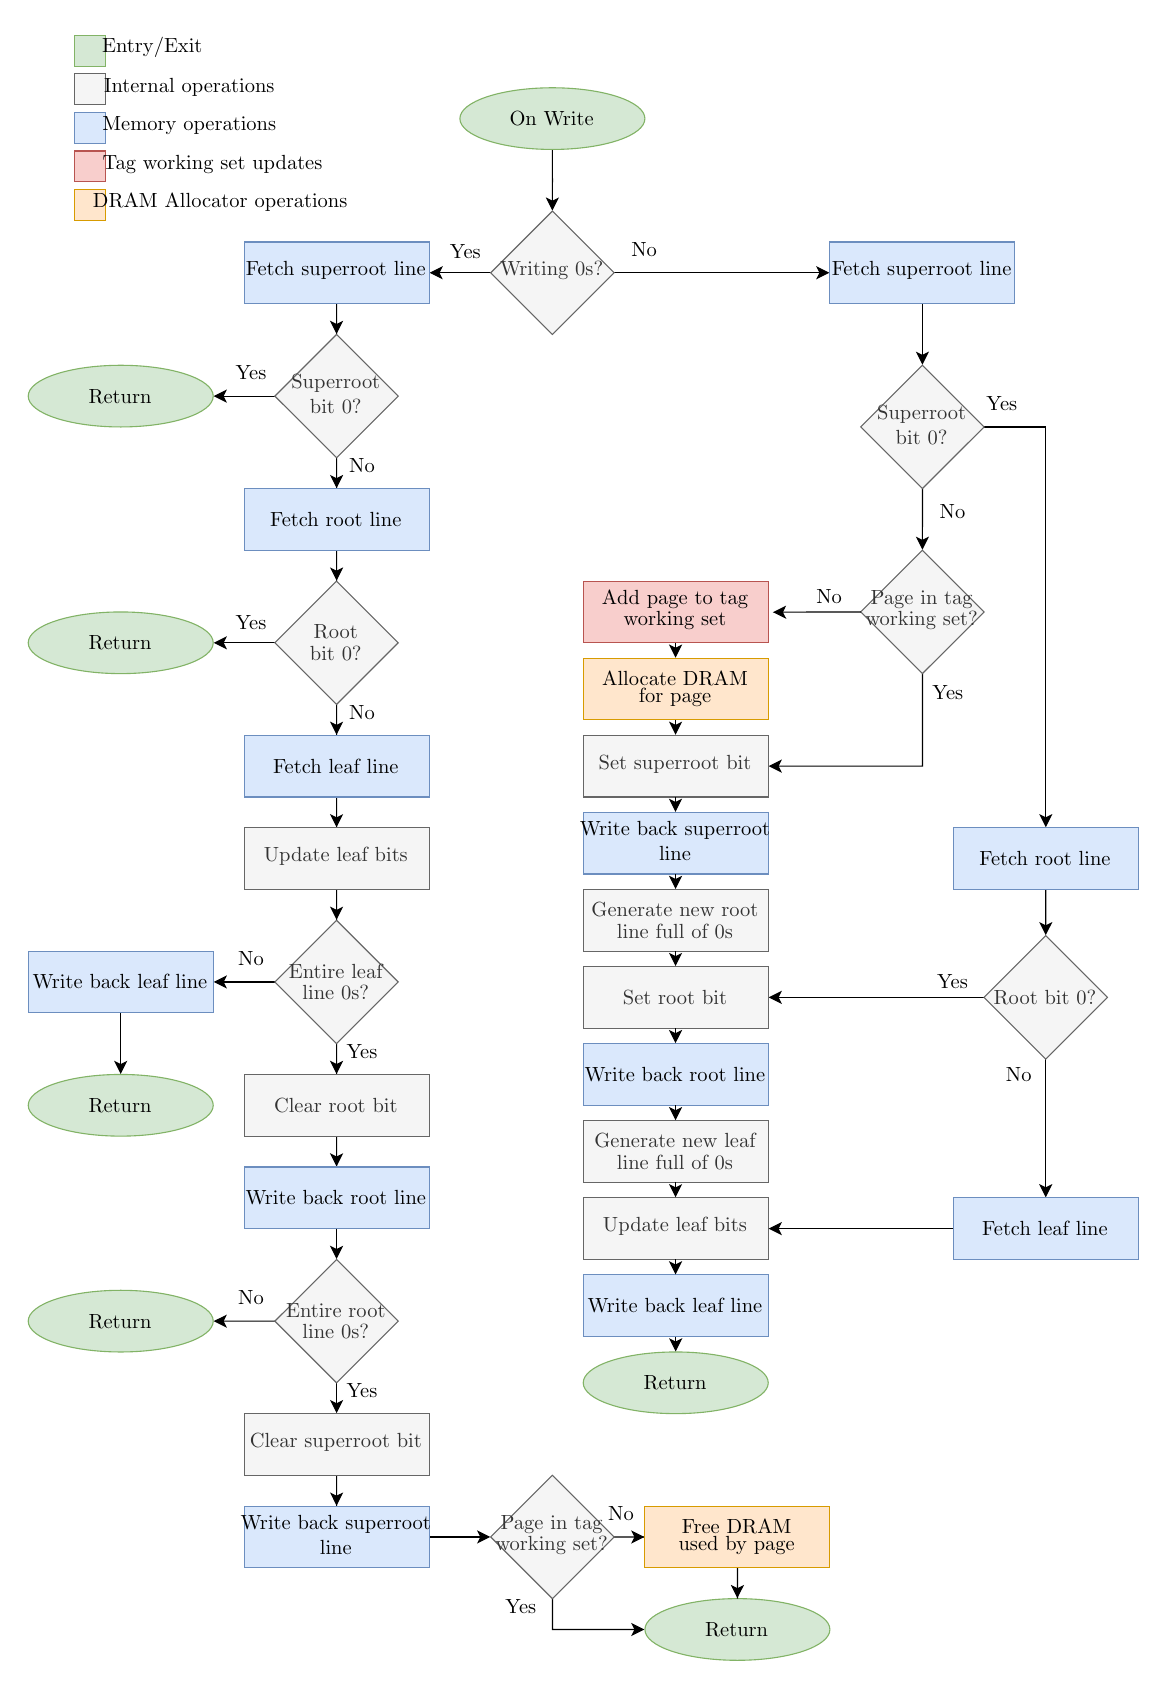
\begin{tikzpicture}[y=1cm, x=1cm, yscale=\globalscale,xscale=\globalscale, every node/.append style={scale=\globalscale}, inner sep=0pt, outer sep=0pt]
  \path[draw=black,miter limit=10.0] (8.9958, 25.9556) -- (8.9966, 25.4257) -- (8.9961, 25.0658);



  \path[draw=black,fill=black,miter limit=10.0] (8.9958, 24.9269) -- (8.9035, 25.1121) -- (8.9961, 25.0658) -- (9.0887, 25.1119) -- cycle;



  \path[draw=c82b366,fill=cd5e8d4] (8.9958, 26.4848) ellipse (1.5875cm and 0.5292cm);



  \begin{scope}[fill=black,anchor=south]
    \node[text=black,anchor=south] (text5734) at (8.9826, 26.3657){On Write};



  \end{scope}
  \path[draw=black,miter limit=10.0] (10.0542, 23.839) -- (13.5898, 23.839);



  \path[draw=black,fill=black,miter limit=10.0] (13.7287, 23.839) -- (13.5435, 23.7464) -- (13.5898, 23.839) -- (13.5435, 23.9316) -- cycle;



  \path[draw=black,miter limit=10.0] (7.9375, 23.839) -- (7.0477, 23.839);



  \path[draw=black,fill=black,miter limit=10.0] (6.9088, 23.839) -- (7.094, 23.9316) -- (7.0477, 23.839) -- (7.094, 23.7464) -- cycle;



  \path[draw=c666666,fill=whitesmoke,miter limit=10.0] (8.9958, 24.8973) -- (10.0542, 23.839) -- (8.9958, 22.7806) -- (7.9375, 23.839) -- cycle;



  \begin{scope}[fill=c333333,anchor=south]
    \node[text=c333333,anchor=south] (text5927) at (8.9826, 23.7199){Writing 0s?};



  \end{scope}
  \path (9.7896, 24.6327) rectangle (11.3771, 23.839);



  \begin{scope}[fill=black,anchor=south]
    \node[text=black,anchor=south] (text4003) at (10.5701, 24.1168){No};



  \end{scope}
  \path[draw=c82b366,fill=cd5e8d4] (0.7938, 27.9135) rectangle (1.3229, 27.3844);



  \path (1.2171, 28.0458) rectangle (3.0692, 27.2521);



  \begin{scope}[fill=black,anchor=south]
    \node[text=black,anchor=south] (text5941) at (2.1299, 27.5299){Entry/Exit};



  \end{scope}
  \path[draw=c666666,fill=whitesmoke] (0.7938, 27.2521) rectangle (1.3229, 26.7229);



  \path (1.1906, 27.3844) rectangle (4.3656, 26.5906);



  \begin{scope}[fill=black,anchor=south]
    \node[text=black,anchor=south] (text8471) at (2.7649, 26.8684){Internal operations};



  \end{scope}
  \path[draw=c6c8ebf,fill=cdae8fc] (0.7938, 26.5906) rectangle (1.3229, 26.0615);



  \path (1.0583, 26.7229) rectangle (4.4979, 25.9292);



  \begin{scope}[fill=black,anchor=south]
    \node[text=black,anchor=south] (text6606) at (2.7649, 26.207){Memory operations};



  \end{scope}
  \path[draw=black,miter limit=10.0] (15.3458, 23.3098) -- (15.3458, 22.42);



  \path[draw=black,fill=black,miter limit=10.0] (15.3458, 22.2811) -- (15.2532, 22.4663) -- (15.3458, 22.42) -- (15.4384, 22.4663) -- cycle;



  \path[draw=c6c8ebf,fill=cdae8fc] (13.7583, 24.3681) rectangle (16.9333, 23.3098);



  \begin{scope}[fill=black,anchor=south]
    \node[text=black,anchor=south] (text4133) at (15.3326, 23.7199){Fetch superroot line};



  \end{scope}
  \path[draw=black,miter limit=10.0] (15.3466, 20.1356) -- (15.3466, 19.6048) -- (15.3461, 19.245);



  \path[draw=black,fill=black,miter limit=10.0] (15.3458, 19.1061) -- (15.2535, 19.2913) -- (15.3461, 19.245) -- (15.4387, 19.291) -- cycle;



  \path[draw=black,miter limit=10.0] (16.4034, 21.1923) -- (17.4633, 21.1923) -- (17.4633, 14.4825);



  \path[draw=black,fill=black,miter limit=10.0] (17.4633, 14.3436) -- (17.3707, 14.5288) -- (17.4633, 14.4825) -- (17.5559, 14.5288) -- cycle;



  \path[draw=c666666,fill=whitesmoke,miter limit=10.0] (15.3458, 22.2515) -- (16.4042, 21.1931) -- (15.3458, 20.1348) -- (14.2875, 21.1931) -- cycle;



  \begin{scope}[fill=c333333,anchor=south]
    \node[text=c333333,anchor=south] (text4247) at (15.3326, 21.2593){Superroot};



    \node[text=c333333,anchor=south] (text1659) at (15.3326, 20.8889){bit 0?};



  \end{scope}
  \path (15.9279, 21.9869) rectangle (17.5154, 21.1931);



  \begin{scope}[fill=black,anchor=south]
    \node[text=black,anchor=south] (text9686) at (16.7084, 21.4709){Yes};



  \end{scope}
  \path (15.0813, 20.1348) rectangle (16.6688, 19.341);



  \begin{scope}[fill=black,anchor=south]
    \node[text=black,anchor=south] (text7678) at (15.8618, 19.6189){No};



  \end{scope}
  \path (15.0813, 12.065) rectangle (16.6688, 11.2712);



  \begin{scope}[fill=black,anchor=south]
    \node[text=black,anchor=south] (text6855) at (15.8618, 11.5491){Yes};



  \end{scope}
  \path[draw=cb85450,fill=cf8cecc] (9.525, 18.5473) rectangle (12.7, 17.489);



  \begin{scope}[fill=black,anchor=south]
    \node[text=black,anchor=south] (text5522) at (11.0993, 18.0843){Add page to tag};



    \node[text=black,anchor=south] (text964) at (11.0993, 17.7139){working set};



  \end{scope}
  \path (12.9646, 18.6796) rectangle (14.5521, 17.8858);



  \begin{scope}[fill=black,anchor=south]
    \node[text=black,anchor=south] (text7224) at (13.7451, 18.1636){No};



  \end{scope}
  \path[draw=c82b366,fill=cd5e8d4] (11.1125, 4.789) ellipse (1.5875cm and 0.5292cm);



  \begin{scope}[fill=black,anchor=south]
    \node[text=black,anchor=south] (text3782) at (11.0993, 4.6699){Return};



  \end{scope}
  \path[draw=black,miter limit=10.0] (15.3466, 16.9606) -- (15.3466, 15.3715) -- (12.8685, 15.3723);



  \path[draw=black,fill=black,miter limit=10.0] (12.7296, 15.3723) -- (12.9148, 15.4649) -- (12.8685, 15.3723) -- (12.9148, 15.2797) -- cycle;



  \path[draw=c666666,fill=whitesmoke,miter limit=10.0] (15.3458, 19.0765) -- (16.4042, 18.0181) -- (15.3458, 16.9598) -- (14.2875, 18.0181) -- cycle;



  \begin{scope}[fill=c333333,anchor=south]
    \node[text=c333333,anchor=south] (text1397) at (15.3326, 18.0843){Page in tag};



    \node[text=c333333,anchor=south] (text872) at (15.3326, 17.7139){working set?};



  \end{scope}
  \path[draw=black,miter limit=10.0] (14.2883, 18.0173) -- (13.4945, 18.0173) -- (12.9416, 18.0139);



  \path[draw=black,fill=black,miter limit=10.0] (12.8027, 18.0131) -- (12.9873, 18.1068) -- (12.9416, 18.0139) -- (12.9884, 17.9216) -- cycle;



  \path[draw=black,miter limit=10.0] (16.4042, 11.4035) -- (12.8685, 11.4035);



  \path[draw=black,fill=black,miter limit=10.0] (12.7296, 11.4035) -- (12.9148, 11.4961) -- (12.8685, 11.4035) -- (12.9148, 11.3109) -- cycle;



  \path[draw=black,miter limit=10.0] (17.4625, 10.3452) -- (17.4625, 8.1325);



  \path[draw=black,fill=black,miter limit=10.0] (17.4625, 7.9936) -- (17.3699, 8.1788) -- (17.4625, 8.1325) -- (17.5551, 8.1788) -- cycle;



  \path[draw=c666666,fill=whitesmoke,miter limit=10.0] (17.4625, 12.4619) -- (18.5208, 11.4035) -- (17.4625, 10.3452) -- (16.4042, 11.4035) -- cycle;



  \begin{scope}[fill=c333333,anchor=south]
    \node[text=c333333,anchor=south] (text1893) at (17.4493, 11.2845){Root bit 0?};



  \end{scope}
  \path[draw=cd79b00,fill=cffe6cc] (9.525, 17.2244) rectangle (12.7, 16.166);



  \begin{scope}[fill=black,anchor=south]
    \node[text=black,anchor=south] (text5036) at (11.0993, 16.7614){Allocate DRAM};



    \node[text=black,anchor=south] (text6463) at (11.0993, 16.3909){for page};



  \end{scope}
  \path[draw=cb85450,fill=cf8cecc] (0.7938, 25.9292) rectangle (1.3229, 25.4);



  \path (1.1906, 26.0615) rectangle (5.1594, 25.2677);



  \begin{scope}[fill=black,anchor=south]
    \node[text=black,anchor=south] (text7397) at (3.1618, 25.5455){Tag working set updates};



  \end{scope}
  \path[draw=c666666,fill=whitesmoke] (9.525, 15.9015) rectangle (12.7, 14.8431);



  \begin{scope}[fill=c333333,anchor=south]
    \node[text=c333333,anchor=south] (text8435) at (11.0993, 15.2532){Set superroot bit};



  \end{scope}
  \path[draw=black,miter limit=10.0] (11.1093, 17.489) -- (11.1093, 17.3929);



  \path[draw=black,fill=black,miter limit=10.0] (11.1093, 17.254) -- (11.0167, 17.4392) -- (11.1093, 17.3929) -- (11.2019, 17.4392) -- cycle;



  \path[draw=black,miter limit=10.0] (11.1093, 16.166) -- (11.1093, 16.07);



  \path[draw=black,fill=black,miter limit=10.0] (11.1093, 15.9311) -- (11.0167, 16.1163) -- (11.1093, 16.07) -- (11.2019, 16.1163) -- cycle;



  \path[draw=c6c8ebf,fill=cdae8fc] (9.525, 14.5785) rectangle (12.7, 13.5202);



  \begin{scope}[fill=black,anchor=south]
    \node[text=black,anchor=south] (text6466) at (11.0993, 14.1155){Write back superroot};



    \node[text=black,anchor=south] (text3014) at (11.0993, 13.7451){line};



  \end{scope}
  \path[draw=black,miter limit=10.0] (11.1093, 14.8431) -- (11.1093, 14.7471);



  \path[draw=black,fill=black,miter limit=10.0] (11.1093, 14.6082) -- (11.0167, 14.7934) -- (11.1093, 14.7471) -- (11.2019, 14.7934) -- cycle;



  \path[draw=c666666,fill=whitesmoke] (9.525, 13.2556) rectangle (12.7, 12.1973);



  \begin{scope}[fill=c333333,anchor=south]
    \node[text=c333333,anchor=south] (text5640) at (11.0993, 12.7926){Generate new root};



    \node[text=c333333,anchor=south] (text3271) at (11.0993, 12.4222){line full of 0s};



  \end{scope}
  \path[draw=black,miter limit=10.0] (11.1093, 13.5202) -- (11.1093, 13.4242);



  \path[draw=black,fill=black,miter limit=10.0] (11.1093, 13.2853) -- (11.0167, 13.4705) -- (11.1093, 13.4242) -- (11.2019, 13.4705) -- cycle;



  \path[draw=c666666,fill=whitesmoke] (9.525, 11.9327) rectangle (12.7, 10.8744);



  \begin{scope}[fill=c333333,anchor=south]
    \node[text=c333333,anchor=south] (text4159) at (11.0993, 11.2845){Set root bit};



  \end{scope}
  \path[draw=black,miter limit=10.0] (11.1093, 12.1973) -- (11.1093, 12.1012);



  \path[draw=black,fill=black,miter limit=10.0] (11.1093, 11.9623) -- (11.0167, 12.1475) -- (11.1093, 12.1012) -- (11.2019, 12.1475) -- cycle;



  \path[draw=c6c8ebf,fill=cdae8fc] (9.525, 10.6098) rectangle (12.7, 9.5515);



  \begin{scope}[fill=black,anchor=south]
    \node[text=black,anchor=south] (text2665) at (11.0993, 9.9616){Write back root line};



  \end{scope}
  \path[draw=black,miter limit=10.0] (11.1093, 10.8744) -- (11.1093, 10.7783);



  \path[draw=black,fill=black,miter limit=10.0] (11.1093, 10.6394) -- (11.0167, 10.8246) -- (11.1093, 10.7783) -- (11.2019, 10.8246) -- cycle;



  \path[draw=c666666,fill=whitesmoke] (9.525, 9.2869) rectangle (12.7, 8.2285);



  \begin{scope}[fill=c333333,anchor=south]
    \node[text=c333333,anchor=south] (text6195) at (11.0993, 8.8239){Generate new leaf};



    \node[text=c333333,anchor=south] (text9396) at (11.0993, 8.4534){line full of 0s};



  \end{scope}
  \path[draw=black,miter limit=10.0] (11.1093, 9.5515) -- (11.1093, 9.4554);



  \path[draw=black,fill=black,miter limit=10.0] (11.1093, 9.3165) -- (11.0167, 9.5017) -- (11.1093, 9.4554) -- (11.2019, 9.5017) -- cycle;



  \path[draw=c666666,fill=whitesmoke] (9.525, 7.964) rectangle (12.7, 6.9056);



  \begin{scope}[fill=c333333,anchor=south]
    \node[text=c333333,anchor=south] (text2634) at (11.0993, 7.3157){Update leaf bits};



  \end{scope}
  \path[draw=black,miter limit=10.0] (11.1093, 8.2285) -- (11.1093, 8.1325);



  \path[draw=black,fill=black,miter limit=10.0] (11.1093, 7.9936) -- (11.0167, 8.1788) -- (11.1093, 8.1325) -- (11.2019, 8.1788) -- cycle;



  \path[draw=c6c8ebf,fill=cdae8fc] (9.525, 6.641) rectangle (12.7, 5.5827);



  \begin{scope}[fill=black,anchor=south]
    \node[text=black,anchor=south] (text9109) at (11.0993, 5.9928){Write back leaf line};



  \end{scope}
  \path[draw=black,miter limit=10.0] (11.1093, 6.9056) -- (11.1093, 6.8096);



  \path[draw=black,fill=black,miter limit=10.0] (11.1093, 6.6707) -- (11.0167, 6.8559) -- (11.1093, 6.8096) -- (11.2019, 6.8559) -- cycle;



  \path[draw=black,miter limit=10.0] (11.1117, 5.5827) -- (11.1117, 5.4867);



  \path[draw=black,fill=black,miter limit=10.0] (11.1117, 5.3478) -- (11.0191, 5.533) -- (11.1117, 5.4867) -- (11.2043, 5.533) -- cycle;



  \path[draw=black,miter limit=10.0] (17.4633, 13.2556) -- (17.4633, 12.7257) -- (17.4633, 12.9902) -- (17.4628, 12.6304);



  \path[draw=black,fill=black,miter limit=10.0] (17.4625, 12.4915) -- (17.3702, 12.6767) -- (17.4628, 12.6304) -- (17.5554, 12.6765) -- cycle;



  \path[draw=c6c8ebf,fill=cdae8fc] (15.875, 14.314) rectangle (19.05, 13.2556);



  \begin{scope}[fill=black,anchor=south]
    \node[text=black,anchor=south] (text4820) at (17.4493, 13.6657){Fetch root line};



  \end{scope}
  \path[draw=black,miter limit=10.0] (15.875, 7.4348) -- (12.8685, 7.4348);



  \path[draw=black,fill=black,miter limit=10.0] (12.7296, 7.4348) -- (12.9148, 7.5274) -- (12.8685, 7.4348) -- (12.9148, 7.3422) -- cycle;



  \path[draw=c6c8ebf,fill=cdae8fc] (15.875, 7.964) rectangle (19.05, 6.9056);



  \begin{scope}[fill=black,anchor=south]
    \node[text=black,anchor=south] (text1073) at (17.4493, 7.3157){Fetch leaf line};



  \end{scope}
  \path (16.219, 10.4775) rectangle (17.8065, 9.6837);



  \begin{scope}[fill=black,anchor=south]
    \node[text=black,anchor=south] (text4870) at (16.9995, 9.9616){No};



  \end{scope}
  \path (15.0019, 17.0392) rectangle (16.5894, 16.2454);



  \begin{scope}[fill=black,anchor=south]
    \node[text=black,anchor=south] (text101) at (15.7824, 16.5232){Yes};



  \end{scope}
  \path[draw=black,miter limit=10.0] (5.2925, 23.3098) -- (5.2925, 22.7798) -- (5.2925, 23.309) -- (5.2919, 22.9492);



  \path[draw=black,fill=black,miter limit=10.0] (5.2917, 22.8103) -- (5.1993, 22.9955) -- (5.2919, 22.9492) -- (5.3845, 22.9952) -- cycle;



  \path[draw=c6c8ebf,fill=cdae8fc] (3.7042, 24.3681) rectangle (6.8792, 23.3098);



  \begin{scope}[fill=black,anchor=south]
    \node[text=black,anchor=south] (text834) at (5.2784, 23.7199){Fetch superroot line};



  \end{scope}
  \path (6.7204, 24.6062) rectangle (8.3079, 23.8125);



  \begin{scope}[fill=black,anchor=south]
    \node[text=black,anchor=south] (text2552) at (7.5009, 24.0903){Yes};



  \end{scope}
  \path[draw=black,miter limit=10.0] (5.2925, 20.6648) -- (5.2925, 20.134) -- (5.2925, 20.6632) -- (5.2919, 20.3033);



  \path[draw=black,fill=black,miter limit=10.0] (5.2917, 20.1644) -- (5.1993, 20.3496) -- (5.2919, 20.3033) -- (5.3845, 20.3494) -- cycle;



  \path[draw=black,miter limit=10.0] (4.2333, 21.7223) -- (3.3435, 21.7223);



  \path[draw=black,fill=black,miter limit=10.0] (3.2046, 21.7223) -- (3.3898, 21.8149) -- (3.3435, 21.7223) -- (3.3898, 21.6297) -- cycle;



  \path[draw=c666666,fill=whitesmoke,miter limit=10.0] (5.2917, 22.7806) -- (6.35, 21.7223) -- (5.2917, 20.664) -- (4.2333, 21.7223) -- cycle;



  \begin{scope}[fill=c333333,anchor=south]
    \node[text=c333333,anchor=south] (text214) at (5.2784, 21.7884){Superroot};



    \node[text=c333333,anchor=south] (text8862) at (5.2784, 21.418){bit 0?};



  \end{scope}
  \path[draw=c82b366,fill=cd5e8d4] (1.5875, 21.7223) ellipse (1.5875cm and 0.5292cm);



  \begin{scope}[fill=black,anchor=south]
    \node[text=black,anchor=south] (text3737) at (1.5743, 21.6032){Return};



  \end{scope}
  \path (3.0427, 22.516) rectangle (4.6302, 21.7223);



  \begin{scope}[fill=black,anchor=south]
    \node[text=black,anchor=south] (text291) at (3.8232, 22.0001){Yes};



  \end{scope}
  \path[draw=black,miter limit=10.0] (5.2925, 19.0765) -- (5.2925, 18.5465) -- (5.2925, 19.0757) -- (5.2919, 18.7158);



  \path[draw=black,fill=black,miter limit=10.0] (5.2917, 18.5769) -- (5.1993, 18.7621) -- (5.2919, 18.7158) -- (5.3845, 18.7619) -- cycle;



  \path[draw=c6c8ebf,fill=cdae8fc] (3.7042, 20.1348) rectangle (6.8792, 19.0765);



  \begin{scope}[fill=black,anchor=south]
    \node[text=black,anchor=south] (text1156) at (5.2784, 19.4866){Fetch root line};



  \end{scope}
  \path[draw=black,miter limit=10.0] (5.2925, 16.4314) -- (5.2925, 15.9007) -- (5.2925, 16.4298) -- (5.2919, 16.07);



  \path[draw=black,fill=black,miter limit=10.0] (5.2917, 15.9311) -- (5.1993, 16.1163) -- (5.2919, 16.07) -- (5.3845, 16.116) -- cycle;



  \path[draw=black,miter limit=10.0] (4.2333, 17.489) -- (3.3435, 17.489);



  \path[draw=black,fill=black,miter limit=10.0] (3.2046, 17.489) -- (3.3898, 17.5816) -- (3.3435, 17.489) -- (3.3898, 17.3964) -- cycle;



  \path[draw=c666666,fill=whitesmoke,miter limit=10.0] (5.2917, 18.5473) -- (6.35, 17.489) -- (5.2917, 16.4306) -- (4.2333, 17.489) -- cycle;



  \begin{scope}[fill=c333333,anchor=south]
    \node[text=c333333,anchor=south] (text7042) at (5.2784, 17.5551){Root};



    \node[text=c333333,anchor=south] (text6257) at (5.2784, 17.1847){bit 0?};



  \end{scope}
  \path[draw=c82b366,fill=cd5e8d4] (1.5875, 17.489) ellipse (1.5875cm and 0.5292cm);



  \begin{scope}[fill=black,anchor=south]
    \node[text=black,anchor=south] (text9133) at (1.5743, 17.3699){Return};



  \end{scope}
  \path (3.0427, 18.2298) rectangle (4.6302, 17.436);



  \begin{scope}[fill=black,anchor=south]
    \node[text=black,anchor=south] (text6070) at (3.8232, 17.7139){Yes};



  \end{scope}
  \path[draw=black,miter limit=10.0] (5.2925, 14.8431) -- (5.2925, 14.3132) -- (5.2925, 14.8423) -- (5.2919, 14.4825);



  \path[draw=black,fill=black,miter limit=10.0] (5.2917, 14.3436) -- (5.1993, 14.5288) -- (5.2919, 14.4825) -- (5.3845, 14.5285) -- cycle;



  \path[draw=c6c8ebf,fill=cdae8fc] (3.7042, 15.9015) rectangle (6.8792, 14.8431);



  \begin{scope}[fill=black,anchor=south]
    \node[text=black,anchor=south] (text5603) at (5.2784, 15.2532){Fetch leaf line};



  \end{scope}
  \path[draw=black,miter limit=10.0] (5.2925, 13.2556) -- (5.2925, 12.7257) -- (5.2925, 13.2548) -- (5.2919, 12.895);



  \path[draw=black,fill=black,miter limit=10.0] (5.2917, 12.7561) -- (5.1993, 12.9413) -- (5.2919, 12.895) -- (5.3845, 12.941) -- cycle;



  \path[draw=c666666,fill=whitesmoke] (3.7042, 14.314) rectangle (6.8792, 13.2556);



  \begin{scope}[fill=c333333,anchor=south]
    \node[text=c333333,anchor=south] (text5357) at (5.2784, 13.6657){Update leaf bits};



  \end{scope}
  \path[draw=black,miter limit=10.0] (4.2333, 11.6681) -- (3.3435, 11.6681);



  \path[draw=black,fill=black,miter limit=10.0] (3.2046, 11.6681) -- (3.3898, 11.7607) -- (3.3435, 11.6681) -- (3.3898, 11.5755) -- cycle;



  \path[draw=black,miter limit=10.0] (5.2925, 10.6106) -- (5.2925, 10.0798) -- (5.2925, 10.609) -- (5.2919, 10.2492);



  \path[draw=black,fill=black,miter limit=10.0] (5.2917, 10.1103) -- (5.1993, 10.2955) -- (5.2919, 10.2492) -- (5.3845, 10.2952) -- cycle;



  \path[draw=c666666,fill=whitesmoke,miter limit=10.0] (5.2917, 12.7265) -- (6.35, 11.6681) -- (5.2917, 10.6098) -- (4.2333, 11.6681) -- cycle;



  \begin{scope}[fill=c333333,anchor=south]
    \node[text=c333333,anchor=south] (text4066) at (5.2784, 11.7343){Entire leaf};



    \node[text=c333333,anchor=south] (text5687) at (5.2784, 11.3639){line 0s?};



  \end{scope}
  \path[draw=c82b366,fill=cd5e8d4] (1.5875, 9.5515) ellipse (1.5875cm and 0.5292cm);



  \begin{scope}[fill=black,anchor=south]
    \node[text=black,anchor=south] (text404) at (1.5743, 9.4324){Return};



  \end{scope}
  \path (3.0427, 12.4619) rectangle (4.6302, 11.6681);



  \begin{scope}[fill=black,anchor=south]
    \node[text=black,anchor=south] (text9090) at (3.8232, 11.9459){No};



  \end{scope}
  \path[draw=black,miter limit=10.0] (1.5875, 11.139) -- (1.5875, 10.2492);



  \path[draw=black,fill=black,miter limit=10.0] (1.5875, 10.1103) -- (1.4949, 10.2955) -- (1.5875, 10.2492) -- (1.6801, 10.2955) -- cycle;



  \path[draw=c6c8ebf,fill=cdae8fc] (0.0, 12.1973) rectangle (3.175, 11.139);



  \begin{scope}[fill=black,anchor=south]
    \node[text=black,anchor=south] (text5019) at (1.5743, 11.5491){Write back leaf line};



  \end{scope}
  \path (4.9477, 10.8744) rectangle (6.5352, 10.0806);



  \begin{scope}[fill=black,anchor=south]
    \node[text=black,anchor=south] (text1479) at (5.7282, 10.3584){Yes};



  \end{scope}
  \path[draw=black,miter limit=10.0] (5.2925, 9.0223) -- (5.2925, 8.4923) -- (5.2925, 9.0215) -- (5.2919, 8.6617);



  \path[draw=black,fill=black,miter limit=10.0] (5.2917, 8.5228) -- (5.1993, 8.708) -- (5.2919, 8.6617) -- (5.3845, 8.7077) -- cycle;



  \path[draw=c666666,fill=whitesmoke] (3.7042, 10.0806) rectangle (6.8792, 9.0223);



  \begin{scope}[fill=c333333,anchor=south]
    \node[text=c333333,anchor=south] (text4092) at (5.2784, 9.4324){Clear root bit};



  \end{scope}
  \path (4.9477, 16.6952) rectangle (6.5352, 15.9015);



  \begin{scope}[fill=black,anchor=south]
    \node[text=black,anchor=south] (text4691) at (5.7282, 16.1793){No};



  \end{scope}
  \path[draw=c6c8ebf,fill=cdae8fc] (3.7042, 8.4931) rectangle (6.8792, 7.4348);



  \begin{scope}[fill=black,anchor=south]
    \node[text=black,anchor=south] (text6862) at (5.2784, 7.8449){Write back root line};



  \end{scope}
  \path[draw=black,miter limit=10.0] (5.2917, 7.4348) -- (5.2917, 7.0742);



  \path[draw=black,fill=black,miter limit=10.0] (5.2917, 6.9353) -- (5.1991, 7.1205) -- (5.2917, 7.0742) -- (5.3843, 7.1205) -- cycle;



  \path[draw=black,miter limit=10.0] (4.2341, 5.8465) -- (3.705, 5.8465) -- (3.3435, 5.847);



  \path[draw=black,fill=black,miter limit=10.0] (3.2046, 5.8473) -- (3.3898, 5.9396) -- (3.3435, 5.847) -- (3.3896, 5.7544) -- cycle;



  \path[draw=black,miter limit=10.0] (5.2925, 4.7898) -- (5.2925, 4.4275);



  \path[draw=black,fill=black,miter limit=10.0] (5.2925, 4.2886) -- (5.1999, 4.4738) -- (5.2925, 4.4275) -- (5.3851, 4.4738) -- cycle;



  \path[draw=c666666,fill=whitesmoke,miter limit=10.0] (5.2917, 6.9056) -- (6.35, 5.8473) -- (5.2917, 4.789) -- (4.2333, 5.8473) -- cycle;



  \begin{scope}[fill=c333333,anchor=south]
    \node[text=c333333,anchor=south] (text6997) at (5.2784, 5.9134){Entire root};



    \node[text=c333333,anchor=south] (text2226) at (5.2784, 5.543){line 0s?};



  \end{scope}
  \path (3.0427, 6.641) rectangle (4.6302, 5.8473);



  \begin{scope}[fill=black,anchor=south]
    \node[text=black,anchor=south] (text1230) at (3.8232, 6.1251){No};



  \end{scope}
  \path (4.9477, 5.0535) rectangle (6.5352, 4.2598);



  \begin{scope}[fill=black,anchor=south]
    \node[text=black,anchor=south] (text9915) at (5.7282, 4.5376){Yes};



  \end{scope}
  \path[draw=c82b366,fill=cd5e8d4] (1.5875, 5.8473) ellipse (1.5875cm and 0.5292cm);



  \begin{scope}[fill=black,anchor=south]
    \node[text=black,anchor=south] (text3689) at (1.5743, 5.7282){Return};



  \end{scope}
  \path[draw=black,miter limit=10.0] (5.2925, 3.2015) -- (5.2925, 2.6715) -- (5.2925, 3.2007) -- (5.2919, 2.8408);



  \path[draw=black,fill=black,miter limit=10.0] (5.2917, 2.7019) -- (5.1993, 2.8871) -- (5.2919, 2.8408) -- (5.3845, 2.8869) -- cycle;



  \path[draw=c666666,fill=whitesmoke] (3.7042, 4.2598) rectangle (6.8792, 3.2015);



  \begin{scope}[fill=c333333,anchor=south]
    \node[text=c333333,anchor=south] (text2187) at (5.2784, 3.6116){Clear superroot bit};



  \end{scope}
  \path[draw=black,miter limit=10.0] (6.8792, 2.1431) -- (7.769, 2.1431);



  \path[draw=black,fill=black,miter limit=10.0] (7.9079, 2.1431) -- (7.7227, 2.0505) -- (7.769, 2.1431) -- (7.7227, 2.2357) -- cycle;



  \path[draw=c6c8ebf,fill=cdae8fc] (3.7042, 2.6723) rectangle (6.8792, 1.614);



  \begin{scope}[fill=black,anchor=south]
    \node[text=black,anchor=south] (text1511) at (5.2784, 2.2093){Write back superroot};



    \node[text=black,anchor=south] (text4763) at (5.2784, 1.8389){line};



  \end{scope}
  \path[draw=black,miter limit=10.0] (10.0534, 2.1423) -- (10.5841, 2.1423) -- (10.055, 2.1423) -- (10.4148, 2.1429);



  \path[draw=black,fill=black,miter limit=10.0] (10.5537, 2.1431) -- (10.3688, 2.0503) -- (10.4148, 2.1429) -- (10.3685, 2.2355) -- cycle;



  \path[draw=black,miter limit=10.0] (8.9966, 1.0856) -- (8.9966, 0.5548) -- (10.4148, 0.5556);



  \path[draw=black,fill=black,miter limit=10.0] (10.5537, 0.5556) -- (10.3685, 0.463) -- (10.4148, 0.5556) -- (10.3685, 0.6482) -- cycle;



  \path[draw=c666666,fill=whitesmoke,miter limit=10.0] (8.9958, 3.2015) -- (10.0542, 2.1431) -- (8.9958, 1.0848) -- (7.9375, 2.1431) -- cycle;



  \begin{scope}[fill=c333333,anchor=south]
    \node[text=c333333,anchor=south] (text8672) at (8.9826, 2.2093){Page in tag};



    \node[text=c333333,anchor=south] (text4466) at (8.9826, 1.8389){working set?};



  \end{scope}
  \path[draw=c82b366,fill=cd5e8d4] (12.1708, 0.5556) ellipse (1.5875cm and 0.5292cm);



  \begin{scope}[fill=black,anchor=south]
    \node[text=black,anchor=south] (text6134) at (12.1576, 0.4366){Return};



  \end{scope}
  \path[draw=black,miter limit=10.0] (12.1716, 1.614) -- (12.1716, 1.084) -- (12.1716, 1.6132) -- (12.1711, 1.2533);



  \path[draw=black,fill=black,miter limit=10.0] (12.1708, 1.1144) -- (12.0785, 1.2996) -- (12.1711, 1.2533) -- (12.2637, 1.2994) -- cycle;



  \path[draw=cd79b00,fill=cffe6cc] (10.5833, 2.6723) rectangle (13.7583, 1.614);



  \begin{scope}[fill=black,anchor=south]
    \node[text=black,anchor=south] (text5025) at (12.1576, 2.2093){Free DRAM};



    \node[text=black,anchor=south] (text8077) at (12.1576, 1.8389){used by page};



  \end{scope}
  \path (7.6729, 1.3494) rectangle (9.2604, 0.5556);



  \begin{scope}[fill=black,anchor=south]
    \node[text=black,anchor=south] (text4703) at (8.4534, 0.8334){Yes};



  \end{scope}
  \path (9.3927, 2.9369) rectangle (10.9802, 2.1431);



  \begin{scope}[fill=black,anchor=south]
    \node[text=black,anchor=south] (text4053) at (10.1732, 2.4209){No};



  \end{scope}
  \path[draw=cd79b00,fill=cffe6cc] (0.7938, 25.2677) rectangle (1.3229, 24.7385);



  \path (1.0583, 25.4) rectangle (5.5563, 24.6062);



  \begin{scope}[fill=black,anchor=south]
    \node[text=black,anchor=south] (text198) at (3.2941, 24.8841){DRAM Allocator operations};



  \end{scope}
  \path (4.9477, 20.9285) rectangle (6.5352, 20.1348);



  \begin{scope}[fill=black,anchor=south]
    \node[text=black,anchor=south] (text1854) at (5.7282, 20.4126){No};



  \end{scope}

\end{tikzpicture}
